\newpage
\section{Análisis de Componentes Principales}
\subsection{Enunciado}
Aplicación del PCA: Utilizando Python y las librerías correspondientes (sklearn, pandas, matplotlib, etc.), aplicarán PCA sobre los datos estandarizados.

Análisis 1: Elección de Componentes Principales: Deberán determinar el número 
adecuado de componentes a retener basándose en la varianza explicada acumulada. 
Como pauta: retener los componentes principales que expliquen al menos el 80 por ciento
de la varianza total. Esto suele dar un buen balance entre simplificación y retención 
de la información clave. En este punto se quedara con un número determinado de componentes según el criterio de la varianza total.

Análisis 2: Gráfica Unitaria y Bautizo de Ejes:
Una vez seleccionados los dos primeros componentes, generar una gráfica de dispersión 
(scatter plot) en dos dimensiones con los datos proyectados en el espacio definido por 
los primeros dos componentes principales. Interpretar qué representa cada eje en 
función de las variables originales. Basado en las cargas de las variables en cada componente, asignar nombres descriptivos a los ejes (por ejemplo, “Eficiencia Operacional” o “Costo de Producción”). En este punto se quedara con 2 componentes.

\subsection{Aplicación del PCA}
Utilizando los datos estandarizados, se procede a aplicar PCA.

\begin{verbatim}
scaler = StandardScaler()
X_scaled = scaler.fit_transform(X)
pca = PCA(n_components=2) 
X_pca = pca.fit_transform(X_scaled)
\end{verbatim}


\subsection{Análisis 1: Elección de Componentes Principales}
\subsubsection{PCA con 2 componentes}
Tomando en cuenta que para este análisis se utilizarán los dos primeros componentes, 
con la gráfica y también se procede a calcular la varianza explicada acumulada.

\begin{figure}[h!]
    \centering
    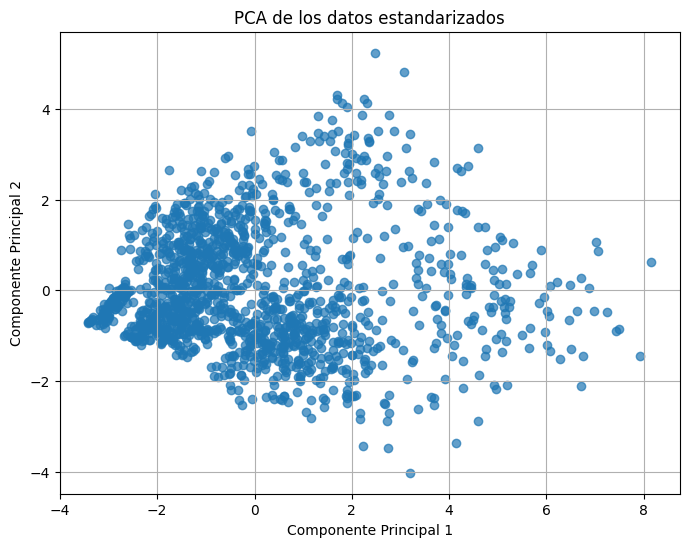
\includegraphics[width=1\textwidth]{images/pca-2-components.png}
    \caption{PCA con los dos primeros componentes}
    \label{fig:pca_2_components}
\end{figure}

Los resultados de la varianza nos muestran que:    
\begin{itemize}
    \item \textbf{Varianza explicada por cada componente:} [0.51429629, 0.19511065]
    \begin{itemize}
        \item El primer componente explica el 51.43\% de la varianza.
        \item El segundo componente explica el 19.51\% de la varianza.
    \end{itemize}

    \item \textbf{Varianza acumulada:} [0.51429629, 0.70940693]
    \begin{itemize}
        \item La suma acumulada de los dos primeros componentes es aproximadamente 71.94\%.
    \end{itemize}
\end{itemize}

Esto nos muestra que los dos primeros componentes explican aproximadamente el 71.94\% de la varianza total, 
pero no son lo suficientemente altos como para retenerlos, por lo cual vamos a probar con 3 componentes.

\subsubsection{PCA con 3 componentes}
Tomando en cuenta que para este análisis se utilizarán los tres primeros componentes.

\begin{verbatim}
pca = PCA(n_components=3) 
X_pca = pca.fit_transform(X_scaled)
\end{verbatim}

Al ser tres componentes, se procede a graficar en 3 dimensiones.

\begin{figure}[H]
    \centering
    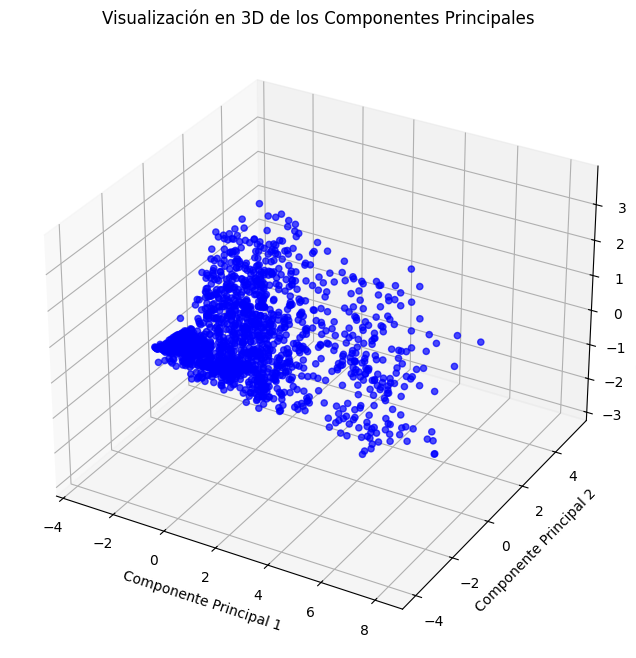
\includegraphics[width=1\textwidth]{images/pca-3-components.png}
    \caption{PCA con los tres primeros componentes}
    \label{fig:pca_3_components}
\end{figure}

Los resultados de la varianza nos muestran que:    
\begin{itemize}
    \item \textbf{Varianza explicada por cada componente:} [0.51429629, 0.19511065, 0.09318736]
    \begin{itemize}
        \item El primer componente explica el 51.43\% de la varianza.
        \item El segundo componente explica el 19.51\% de la varianza.
        \item El tercer componente explica el 9.32\% de la varianza.
    \end{itemize}

    \item \textbf{Varianza acumulada:} [0.51429629 0.70940693 0.80259429]
    \begin{itemize}
        \item La suma acumulada de los dos primeros componentes es aproximadamente 80.26\%.
    \end{itemize}
\end{itemize}

Esto nos muestra que los tres primeros componentes explican aproximadamente el 80.25\% de la varianza total,
y que ellos capturan la mayoría de la información relevante de los datos principales


\subsection{Análisis 2: Gráfica Unitaria y Bautizo de Ejes}